\documentclass[1p]{elsarticle_modified}
%\bibliographystyle{elsarticle-num}

%\usepackage[colorlinks]{hyperref}
%\usepackage{abbrmath_seonhwa} %\Abb, \Ascr, \Acal ,\Abf, \Afrak
\usepackage{amsfonts}
\usepackage{amssymb}
\usepackage{amsmath}
\usepackage{amsthm}
\usepackage{scalefnt}
\usepackage{amsbsy}
\usepackage{kotex}
\usepackage{caption}
\usepackage{subfig}
\usepackage{color}
\usepackage{graphicx}
\usepackage{xcolor} %% white, black, red, green, blue, cyan, magenta, yellow
\usepackage{float}
\usepackage{setspace}
\usepackage{hyperref}

\usepackage{tikz}
\usetikzlibrary{arrows}

\usepackage{multirow}
\usepackage{array} % fixed length table
\usepackage{hhline}

%%%%%%%%%%%%%%%%%%%%%
\makeatletter
\renewcommand*\env@matrix[1][\arraystretch]{%
	\edef\arraystretch{#1}%
	\hskip -\arraycolsep
	\let\@ifnextchar\new@ifnextchar
	\array{*\c@MaxMatrixCols c}}
\makeatother %https://tex.stackexchange.com/questions/14071/how-can-i-increase-the-line-spacing-in-a-matrix
%%%%%%%%%%%%%%%

\usepackage[normalem]{ulem}

\newcommand{\msout}[1]{\ifmmode\text{\sout{\ensuremath{#1}}}\else\sout{#1}\fi}
%SOURCE: \msout is \stkout macro in https://tex.stackexchange.com/questions/20609/strikeout-in-math-mode

\newcommand{\cancel}[1]{
	\ifmmode
	{\color{red}\msout{#1}}
	\else
	{\color{red}\sout{#1}}
	\fi
}

\newcommand{\add}[1]{
	{\color{blue}\uwave{#1}}
}

\newcommand{\replace}[2]{
	\ifmmode
	{\color{red}\msout{#1}}{\color{blue}\uwave{#2}}
	\else
	{\color{red}\sout{#1}}{\color{blue}\uwave{#2}}
	\fi
}

\newcommand{\Sol}{\mathcal{S}} %segment
\newcommand{\D}{D} %diagram
\newcommand{\A}{\mathcal{A}} %arc


%%%%%%%%%%%%%%%%%%%%%%%%%%%%%5 test

\def\sl{\operatorname{\textup{SL}}(2,\Cbb)}
\def\psl{\operatorname{\textup{PSL}}(2,\Cbb)}
\def\quan{\mkern 1mu \triangleright \mkern 1mu}

\theoremstyle{definition}
\newtheorem{thm}{Theorem}[section]
\newtheorem{prop}[thm]{Proposition}
\newtheorem{lem}[thm]{Lemma}
\newtheorem{ques}[thm]{Question}
\newtheorem{cor}[thm]{Corollary}
\newtheorem{defn}[thm]{Definition}
\newtheorem{exam}[thm]{Example}
\newtheorem{rmk}[thm]{Remark}
\newtheorem{alg}[thm]{Algorithm}

\newcommand{\I}{\sqrt{-1}}
\begin{document}

%\begin{frontmatter}
%
%\title{Boundary parabolic representations of knots up to 8 crossings}
%
%%% Group authors per affiliation:
%\author{Yunhi Cho} 
%\address{Department of Mathematics, University of Seoul, Seoul, Korea}
%\ead{yhcho@uos.ac.kr}
%
%
%\author{Seonhwa Kim} %\fnref{s_kim}}
%\address{Center for Geometry and Physics, Institute for Basic Science, Pohang, 37673, Korea}
%\ead{ryeona17@ibs.re.kr}
%
%\author{Hyuk Kim}
%\address{Department of Mathematical Sciences, Seoul National University, Seoul 08826, Korea}
%\ead{hyukkim@snu.ac.kr}
%
%\author{Seokbeom Yoon}
%\address{Department of Mathematical Sciences, Seoul National University, Seoul, 08826,  Korea}
%\ead{sbyoon15@snu.ac.kr}
%
%\begin{abstract}
%We find all boundary parabolic representation of knots up to 8 crossings.
%
%\end{abstract}
%\begin{keyword}
%    \MSC[2010] 57M25 
%\end{keyword}
%
%\end{frontmatter}

%\linenumbers
%\tableofcontents
%
\newcommand\colored[1]{\textcolor{white}{\rule[-0.35ex]{0.8em}{1.4ex}}\kern-0.8em\color{red} #1}%
%\newcommand\colored[1]{\textcolor{white}{ #1}\kern-2.17ex	\textcolor{white}{ #1}\kern-1.81ex	\textcolor{white}{ #1}\kern-2.15ex\color{red}#1	}

{\Large $\underline{12a_{0110}~(K12a_{0110})}$}

\setlength{\tabcolsep}{10pt}
\renewcommand{\arraystretch}{1.6}
\vspace{1cm}\begin{tabular}{m{100pt}>{\centering\arraybackslash}m{274pt}}
\multirow{5}{120pt}{
	\centering
	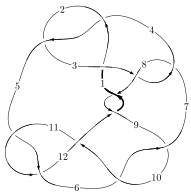
\includegraphics[width=112pt]{../../../GIT/diagram.site/Diagrams/png/911_12a_0110.png}\\
\ \ \ A knot diagram\footnotemark}&
\allowdisplaybreaks
\textbf{Linearized knot diagam} \\
\cline{2-2}
 &
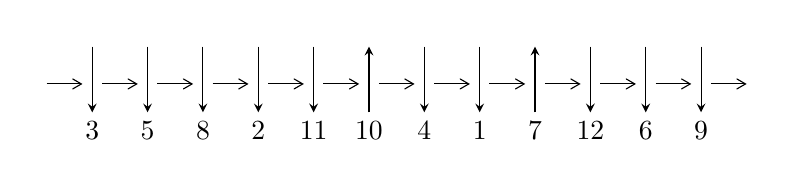
\begin{tikzpicture}[x=20pt, y=17pt]
	% nodes
	\node (C0) at (0, 0) {};
	\node (C1) at (1, 0) {};
	\node (C1U) at (1, +1) {};
	\node (C1D) at (1, -1) {3};

	\node (C2) at (2, 0) {};
	\node (C2U) at (2, +1) {};
	\node (C2D) at (2, -1) {5};

	\node (C3) at (3, 0) {};
	\node (C3U) at (3, +1) {};
	\node (C3D) at (3, -1) {8};

	\node (C4) at (4, 0) {};
	\node (C4U) at (4, +1) {};
	\node (C4D) at (4, -1) {2};

	\node (C5) at (5, 0) {};
	\node (C5U) at (5, +1) {};
	\node (C5D) at (5, -1) {11};

	\node (C6) at (6, 0) {};
	\node (C6U) at (6, +1) {};
	\node (C6D) at (6, -1) {10};

	\node (C7) at (7, 0) {};
	\node (C7U) at (7, +1) {};
	\node (C7D) at (7, -1) {4};

	\node (C8) at (8, 0) {};
	\node (C8U) at (8, +1) {};
	\node (C8D) at (8, -1) {1};

	\node (C9) at (9, 0) {};
	\node (C9U) at (9, +1) {};
	\node (C9D) at (9, -1) {7};

	\node (C10) at (10, 0) {};
	\node (C10U) at (10, +1) {};
	\node (C10D) at (10, -1) {12};

	\node (C11) at (11, 0) {};
	\node (C11U) at (11, +1) {};
	\node (C11D) at (11, -1) {6};

	\node (C12) at (12, 0) {};
	\node (C12U) at (12, +1) {};
	\node (C12D) at (12, -1) {9};
	\node (C13) at (13, 0) {};

	% arrows
	\draw[->,>={angle 60}]
	(C0) edge (C1) (C1) edge (C2) (C2) edge (C3) (C3) edge (C4) (C4) edge (C5) (C5) edge (C6) (C6) edge (C7) (C7) edge (C8) (C8) edge (C9) (C9) edge (C10) (C10) edge (C11) (C11) edge (C12) (C12) edge (C13) ;	\draw[->,>=stealth]
	(C1U) edge (C1D) (C2U) edge (C2D) (C3U) edge (C3D) (C4U) edge (C4D) (C5U) edge (C5D) (C6D) edge (C6U) (C7U) edge (C7D) (C8U) edge (C8D) (C9D) edge (C9U) (C10U) edge (C10D) (C11U) edge (C11D) (C12U) edge (C12D) ;
	\end{tikzpicture} \\
\hhline{~~} \\& 
\textbf{Solving Sequence} \\ \cline{2-2} 
 &
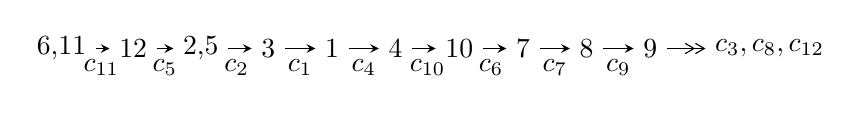
\begin{tikzpicture}[x=23pt, y=7pt]
	% node
	\node (A0) at (-1/8, 0) {6,11};
	\node (A1) at (1, 0) {12};
	\node (A2) at (33/16, 0) {2,5};
	\node (A3) at (25/8, 0) {3};
	\node (A4) at (33/8, 0) {1};
	\node (A5) at (41/8, 0) {4};
	\node (A6) at (49/8, 0) {10};
	\node (A7) at (57/8, 0) {7};
	\node (A8) at (65/8, 0) {8};
	\node (A9) at (73/8, 0) {9};
	\node (C1) at (1/2, -1) {$c_{11}$};
	\node (C2) at (3/2, -1) {$c_{5}$};
	\node (C3) at (21/8, -1) {$c_{2}$};
	\node (C4) at (29/8, -1) {$c_{1}$};
	\node (C5) at (37/8, -1) {$c_{4}$};
	\node (C6) at (45/8, -1) {$c_{10}$};
	\node (C7) at (53/8, -1) {$c_{6}$};
	\node (C8) at (61/8, -1) {$c_{7}$};
	\node (C9) at (69/8, -1) {$c_{9}$};
	\node (A10) at (11, 0) {$c_{3},c_{8},c_{12}$};

	% edge
	\draw[->,>=stealth]	
	(A0) edge (A1) (A1) edge (A2) (A2) edge (A3) (A3) edge (A4) (A4) edge (A5) (A5) edge (A6) (A6) edge (A7) (A7) edge (A8) (A8) edge (A9) ;
	\draw[->>,>={angle 60}]	
	(A9) edge (A10);
\end{tikzpicture} \\ 

\end{tabular} \\

\footnotetext{
The image of knot diagram is generated by the software ``\textbf{Draw programme}" developed by Andrew Bartholomew(\url{http://www.layer8.co.uk/maths/draw/index.htm\#Running-draw}), where we modified some parts for our purpose(\url{https://github.com/CATsTAILs/LinksPainter}).
}\phantom \\ \newline 
\centering \textbf{Ideals for irreducible components\footnotemark of $X_{\text{par}}$} 
 
\begin{align*}
I^u_{1}&=\langle 
2 u^{98}-3 u^{97}+\cdots+b+2,\;2 u^{98}-2 u^{97}+\cdots+a-1,\;u^{99}-2 u^{98}+\cdots+4 u-1\rangle \\
I^u_{2}&=\langle 
- u^8+2 u^6- u^5-2 u^4+u^3- u^2+b+u,\;- u^7+2 u^5- u^4-2 u^3+u^2+a+u-1,\\
\phantom{I^u_{2}}&\phantom{= \langle  }u^9- u^8-2 u^7+3 u^6+u^5-3 u^4+2 u^3- u+1\rangle \\
\\
\end{align*}
\raggedright * 2 irreducible components of $\dim_{\mathbb{C}}=0$, with total 108 representations.\\
\footnotetext{All coefficients of polynomials are rational numbers. But the coefficients are sometimes approximated in decimal forms when there is not enough margin.}
\newpage
\renewcommand{\arraystretch}{1}
\centering \section*{I. $I^u_{1}= \langle 2 u^{98}-3 u^{97}+\cdots+b+2,\;2 u^{98}-2 u^{97}+\cdots+a-1,\;u^{99}-2 u^{98}+\cdots+4 u-1 \rangle$}
\flushleft \textbf{(i) Arc colorings}\\
\begin{tabular}{m{7pt} m{180pt} m{7pt} m{180pt} }
\flushright $a_{6}=$&$\begin{pmatrix}0\\u\end{pmatrix}$ \\
\flushright $a_{11}=$&$\begin{pmatrix}1\\0\end{pmatrix}$ \\
\flushright $a_{12}=$&$\begin{pmatrix}1\\u^2\end{pmatrix}$ \\
\flushright $a_{2}=$&$\begin{pmatrix}-2 u^{98}+2 u^{97}+\cdots+6 u+1\\-2 u^{98}+3 u^{97}+\cdots+7 u-2\end{pmatrix}$ \\
\flushright $a_{5}=$&$\begin{pmatrix}u\\u\end{pmatrix}$ \\
\flushright $a_{3}=$&$\begin{pmatrix}-3 u^{98}+3 u^{97}+\cdots- u^2+10 u\\-3 u^{98}+4 u^{97}+\cdots+11 u-3\end{pmatrix}$ \\
\flushright $a_{1}=$&$\begin{pmatrix}u^{16}-5 u^{14}+11 u^{12}-12 u^{10}+5 u^8+2 u^6-2 u^4+1\\u^{18}-4 u^{16}+7 u^{14}-4 u^{12}-3 u^{10}+6 u^8-2 u^6+u^2\end{pmatrix}$ \\
\flushright $a_{4}=$&$\begin{pmatrix}- u^{98}+u^{97}+\cdots+4 u+1\\- u^{98}+2 u^{97}+\cdots+4 u-1\end{pmatrix}$ \\
\flushright $a_{10}=$&$\begin{pmatrix}- u^2+1\\- u^4\end{pmatrix}$ \\
\flushright $a_{7}=$&$\begin{pmatrix}u^5-2 u^3+u\\u^7- u^5+u\end{pmatrix}$ \\
\flushright $a_{8}=$&$\begin{pmatrix}u^{24}-7 u^{22}+\cdots+5 u^4-1\\u^{26}-6 u^{24}+\cdots+2 u^4- u^2\end{pmatrix}$ \\
\flushright $a_{9}=$&$\begin{pmatrix}- u^8+3 u^6-3 u^4+1\\- u^{10}+2 u^8- u^6-2 u^4+u^2\end{pmatrix}$\\&\end{tabular}
\flushleft \textbf{(ii) Obstruction class $= -1$}\\~\\
\flushleft \textbf{(iii) Cusp Shapes $= -6 u^{98}+7 u^{97}+\cdots+26 u-19$}\\~\\
\newpage\renewcommand{\arraystretch}{1}
\flushleft \textbf{(iv) u-Polynomials at the component}\newline \\
\begin{tabular}{m{50pt}|m{274pt}}
Crossings & \hspace{64pt}u-Polynomials at each crossing \\
\hline $$\begin{aligned}c_{1}\end{aligned}$$&$\begin{aligned}
&u^{99}+44 u^{98}+\cdots+40 u+1
\end{aligned}$\\
\hline $$\begin{aligned}c_{2},c_{4}\end{aligned}$$&$\begin{aligned}
&u^{99}-10 u^{98}+\cdots-8 u+1
\end{aligned}$\\
\hline $$\begin{aligned}c_{3},c_{7}\end{aligned}$$&$\begin{aligned}
&u^{99}+u^{98}+\cdots+1536 u+512
\end{aligned}$\\
\hline $$\begin{aligned}c_{5},c_{11}\end{aligned}$$&$\begin{aligned}
&u^{99}+2 u^{98}+\cdots+4 u+1
\end{aligned}$\\
\hline $$\begin{aligned}c_{6},c_{9}\end{aligned}$$&$\begin{aligned}
&u^{99}+6 u^{98}+\cdots+460 u+77
\end{aligned}$\\
\hline $$\begin{aligned}c_{8},c_{12}\end{aligned}$$&$\begin{aligned}
&u^{99}-8 u^{98}+\cdots+10366 u+565
\end{aligned}$\\
\hline $$\begin{aligned}c_{10}\end{aligned}$$&$\begin{aligned}
&u^{99}+52 u^{98}+\cdots+12 u+1
\end{aligned}$\\
\hline
\end{tabular}\\~\\
\newpage\renewcommand{\arraystretch}{1}
\flushleft \textbf{(v) Riley Polynomials at the component}\newline \\
\begin{tabular}{m{50pt}|m{274pt}}
Crossings & \hspace{64pt}Riley Polynomials at each crossing \\
\hline $$\begin{aligned}c_{1}\end{aligned}$$&$\begin{aligned}
&y^{99}+32 y^{98}+\cdots+756 y-1
\end{aligned}$\\
\hline $$\begin{aligned}c_{2},c_{4}\end{aligned}$$&$\begin{aligned}
&y^{99}-44 y^{98}+\cdots+40 y-1
\end{aligned}$\\
\hline $$\begin{aligned}c_{3},c_{7}\end{aligned}$$&$\begin{aligned}
&y^{99}+57 y^{98}+\cdots-6291456 y-262144
\end{aligned}$\\
\hline $$\begin{aligned}c_{5},c_{11}\end{aligned}$$&$\begin{aligned}
&y^{99}-52 y^{98}+\cdots+12 y-1
\end{aligned}$\\
\hline $$\begin{aligned}c_{6},c_{9}\end{aligned}$$&$\begin{aligned}
&y^{99}+68 y^{98}+\cdots-1083848 y-5929
\end{aligned}$\\
\hline $$\begin{aligned}c_{8},c_{12}\end{aligned}$$&$\begin{aligned}
&y^{99}+72 y^{98}+\cdots-22303944 y-319225
\end{aligned}$\\
\hline $$\begin{aligned}c_{10}\end{aligned}$$&$\begin{aligned}
&y^{99}-8 y^{98}+\cdots+48 y-1
\end{aligned}$\\
\hline
\end{tabular}\\~\\
\newpage\flushleft \textbf{(vi) Complex Volumes and Cusp Shapes}
$$\begin{array}{c|c|c}  
\text{Solutions to }I^u_{1}& \I (\text{vol} + \sqrt{-1}CS) & \text{Cusp shape}\\
 \hline 
\begin{aligned}
u &= \phantom{-}0.798665 + 0.599302 I \\
a &= -0.976827 + 0.577800 I \\
b &= -1.129250 - 0.480015 I\end{aligned}
 & \phantom{-}8.49803 - 4.84511 I & \phantom{-0.000000 } 0 \\ \hline\begin{aligned}
u &= \phantom{-}0.798665 - 0.599302 I \\
a &= -0.976827 - 0.577800 I \\
b &= -1.129250 + 0.480015 I\end{aligned}
 & \phantom{-}8.49803 + 4.84511 I & \phantom{-0.000000 } 0 \\ \hline\begin{aligned}
u &= \phantom{-}1.000350 + 0.050995 I \\
a &= \phantom{-}1.42535 - 0.26072 I \\
b &= \phantom{-}2.27637 - 0.80986 I\end{aligned}
 & -1.67165 + 2.02827 I & \phantom{-0.000000 } 0 \\ \hline\begin{aligned}
u &= \phantom{-}1.000350 - 0.050995 I \\
a &= \phantom{-}1.42535 + 0.26072 I \\
b &= \phantom{-}2.27637 + 0.80986 I\end{aligned}
 & -1.67165 - 2.02827 I & \phantom{-0.000000 } 0 \\ \hline\begin{aligned}
u &= -0.902178 + 0.454400 I \\
a &= \phantom{-}0.0890370 - 0.0234107 I \\
b &= -0.217835 - 0.845633 I\end{aligned}
 & \phantom{-}1.61783 + 2.06558 I & \phantom{-0.000000 } 0 \\ \hline\begin{aligned}
u &= -0.902178 - 0.454400 I \\
a &= \phantom{-}0.0890370 + 0.0234107 I \\
b &= -0.217835 + 0.845633 I\end{aligned}
 & \phantom{-}1.61783 - 2.06558 I & \phantom{-0.000000 } 0 \\ \hline\begin{aligned}
u &= \phantom{-}0.816175 + 0.596584 I \\
a &= \phantom{-}0.90939 - 1.15608 I \\
b &= \phantom{-}2.21727 - 1.25204 I\end{aligned}
 & \phantom{-}6.62627 - 10.84290 I & \phantom{-0.000000 } 0 \\ \hline\begin{aligned}
u &= \phantom{-}0.816175 - 0.596584 I \\
a &= \phantom{-}0.90939 + 1.15608 I \\
b &= \phantom{-}2.21727 + 1.25204 I\end{aligned}
 & \phantom{-}6.62627 + 10.84290 I & \phantom{-0.000000 } 0 \\ \hline\begin{aligned}
u &= -0.788174 + 0.579168 I \\
a &= \phantom{-}0.44309 + 1.67989 I \\
b &= \phantom{-}1.51689 + 1.70812 I\end{aligned}
 & \phantom{-}3.17843 + 4.66485 I & \phantom{-0.000000 } 0 \\ \hline\begin{aligned}
u &= -0.788174 - 0.579168 I \\
a &= \phantom{-}0.44309 - 1.67989 I \\
b &= \phantom{-}1.51689 - 1.70812 I\end{aligned}
 & \phantom{-}3.17843 - 4.66485 I & \phantom{-0.000000 } 0\\
 \hline 
 \end{array}$$\newpage$$\begin{array}{c|c|c}  
\text{Solutions to }I^u_{1}& \I (\text{vol} + \sqrt{-1}CS) & \text{Cusp shape}\\
 \hline 
\begin{aligned}
u &= \phantom{-}0.744914 + 0.605828 I \\
a &= -0.079985 - 1.168900 I \\
b &= \phantom{-}0.962462 - 0.769387 I\end{aligned}
 & \phantom{-}8.65243 + 0.12444 I & \phantom{-0.000000 } 0 \\ \hline\begin{aligned}
u &= \phantom{-}0.744914 - 0.605828 I \\
a &= -0.079985 + 1.168900 I \\
b &= \phantom{-}0.962462 + 0.769387 I\end{aligned}
 & \phantom{-}8.65243 - 0.12444 I & \phantom{-0.000000 } 0 \\ \hline\begin{aligned}
u &= \phantom{-}0.771063 + 0.569620 I \\
a &= \phantom{-}0.119221 - 0.166608 I \\
b &= -0.973643 + 0.658801 I\end{aligned}
 & \phantom{-}1.68918 - 2.26594 I & \phantom{-0.000000 } 0 \\ \hline\begin{aligned}
u &= \phantom{-}0.771063 - 0.569620 I \\
a &= \phantom{-}0.119221 + 0.166608 I \\
b &= -0.973643 - 0.658801 I\end{aligned}
 & \phantom{-}1.68918 + 2.26594 I & \phantom{-0.000000 } 0 \\ \hline\begin{aligned}
u &= -0.752820 + 0.580640 I \\
a &= -1.53562 - 1.14343 I \\
b &= -1.228310 - 0.111363 I\end{aligned}
 & \phantom{-}3.27984 - 0.07370 I & \phantom{-0.000000 } 0 \\ \hline\begin{aligned}
u &= -0.752820 - 0.580640 I \\
a &= -1.53562 + 1.14343 I \\
b &= -1.228310 + 0.111363 I\end{aligned}
 & \phantom{-}3.27984 + 0.07370 I & \phantom{-0.000000 } 0 \\ \hline\begin{aligned}
u &= \phantom{-}0.724168 + 0.607828 I \\
a &= -1.01845 + 1.58478 I \\
b &= -0.599810 + 0.255502 I\end{aligned}
 & \phantom{-}6.89015 + 6.12501 I & \phantom{-0.000000 } 0 \\ \hline\begin{aligned}
u &= \phantom{-}0.724168 - 0.607828 I \\
a &= -1.01845 - 1.58478 I \\
b &= -0.599810 - 0.255502 I\end{aligned}
 & \phantom{-}6.89015 - 6.12501 I & \phantom{-0.000000 } 0 \\ \hline\begin{aligned}
u &= \phantom{-}0.881720 + 0.272848 I \\
a &= -0.91493 + 1.57555 I \\
b &= -1.98406 + 1.50327 I\end{aligned}
 & -2.29107 - 2.61357 I & -12.6816 + 6.4490 I \\ \hline\begin{aligned}
u &= \phantom{-}0.881720 - 0.272848 I \\
a &= -0.91493 - 1.57555 I \\
b &= -1.98406 - 1.50327 I\end{aligned}
 & -2.29107 + 2.61357 I & -12.6816 - 6.4490 I\\
 \hline 
 \end{array}$$\newpage$$\begin{array}{c|c|c}  
\text{Solutions to }I^u_{1}& \I (\text{vol} + \sqrt{-1}CS) & \text{Cusp shape}\\
 \hline 
\begin{aligned}
u &= -0.779849 + 0.465975 I \\
a &= -0.285213 + 0.269799 I \\
b &= -0.574238 - 0.041840 I\end{aligned}
 & \phantom{-}1.26426 + 1.96404 I & \phantom{-0.000000 } 0. - 4.36922 I \\ \hline\begin{aligned}
u &= -0.779849 - 0.465975 I \\
a &= -0.285213 - 0.269799 I \\
b &= -0.574238 + 0.041840 I\end{aligned}
 & \phantom{-}1.26426 - 1.96404 I & \phantom{-0.000000 -}0. + 4.36922 I \\ \hline\begin{aligned}
u &= -1.004260 + 0.453349 I \\
a &= -1.41231 - 0.60811 I \\
b &= -2.44810 - 0.42836 I\end{aligned}
 & \phantom{-}0.71840 + 7.06687 I & \phantom{-0.000000 } 0 \\ \hline\begin{aligned}
u &= -1.004260 - 0.453349 I \\
a &= -1.41231 + 0.60811 I \\
b &= -2.44810 + 0.42836 I\end{aligned}
 & \phantom{-}0.71840 - 7.06687 I & \phantom{-0.000000 } 0 \\ \hline\begin{aligned}
u &= -1.092330 + 0.258588 I \\
a &= -1.57152 - 0.29866 I \\
b &= -2.63399 + 0.06600 I\end{aligned}
 & \phantom{-}0.76961 + 7.47794 I & \phantom{-0.000000 } 0 \\ \hline\begin{aligned}
u &= -1.092330 - 0.258588 I \\
a &= -1.57152 + 0.29866 I \\
b &= -2.63399 - 0.06600 I\end{aligned}
 & \phantom{-}0.76961 - 7.47794 I & \phantom{-0.000000 } 0 \\ \hline\begin{aligned}
u &= -0.837177 + 0.170997 I \\
a &= \phantom{-}1.249710 - 0.553710 I \\
b &= \phantom{-}2.50105 - 0.13181 I\end{aligned}
 & -2.94172 + 0.75427 I & -11.8641 - 8.1427 I \\ \hline\begin{aligned}
u &= -0.837177 - 0.170997 I \\
a &= \phantom{-}1.249710 + 0.553710 I \\
b &= \phantom{-}2.50105 + 0.13181 I\end{aligned}
 & -2.94172 - 0.75427 I & -11.8641 + 8.1427 I \\ \hline\begin{aligned}
u &= -1.125850 + 0.299064 I \\
a &= -0.337223 + 0.090504 I \\
b &= -0.624275 - 0.743573 I\end{aligned}
 & \phantom{-}2.27588 + 1.80560 I & \phantom{-0.000000 } 0 \\ \hline\begin{aligned}
u &= -1.125850 - 0.299064 I \\
a &= -0.337223 - 0.090504 I \\
b &= -0.624275 + 0.743573 I\end{aligned}
 & \phantom{-}2.27588 - 1.80560 I & \phantom{-0.000000 } 0\\
 \hline 
 \end{array}$$\newpage$$\begin{array}{c|c|c}  
\text{Solutions to }I^u_{1}& \I (\text{vol} + \sqrt{-1}CS) & \text{Cusp shape}\\
 \hline 
\begin{aligned}
u &= \phantom{-}0.196053 + 0.799972 I \\
a &= -0.54640 + 2.83269 I \\
b &= -1.02080 + 1.28664 I\end{aligned}
 & \phantom{-}3.58238 + 12.05350 I & -5.58626 - 7.48008 I \\ \hline\begin{aligned}
u &= \phantom{-}0.196053 - 0.799972 I \\
a &= -0.54640 - 2.83269 I \\
b &= -1.02080 - 1.28664 I\end{aligned}
 & \phantom{-}3.58238 - 12.05350 I & -5.58626 + 7.48008 I \\ \hline\begin{aligned}
u &= \phantom{-}0.206728 + 0.789199 I \\
a &= -1.297360 - 0.297194 I \\
b &= -0.041729 - 0.559859 I\end{aligned}
 & \phantom{-}5.64791 + 6.12658 I & -2.76593 - 3.29252 I \\ \hline\begin{aligned}
u &= \phantom{-}0.206728 - 0.789199 I \\
a &= -1.297360 + 0.297194 I \\
b &= -0.041729 + 0.559859 I\end{aligned}
 & \phantom{-}5.64791 - 6.12658 I & -2.76593 + 3.29252 I \\ \hline\begin{aligned}
u &= \phantom{-}1.138850 + 0.353272 I \\
a &= -0.218291 + 0.809760 I \\
b &= -0.919968 + 0.560519 I\end{aligned}
 & -2.92898 - 2.30725 I & \phantom{-0.000000 } 0 \\ \hline\begin{aligned}
u &= \phantom{-}1.138850 - 0.353272 I \\
a &= -0.218291 - 0.809760 I \\
b &= -0.919968 - 0.560519 I\end{aligned}
 & -2.92898 + 2.30725 I & \phantom{-0.000000 } 0 \\ \hline\begin{aligned}
u &= -0.196691 + 0.772888 I \\
a &= -0.90453 - 2.07428 I \\
b &= -1.33709 - 0.77630 I\end{aligned}
 & \phantom{-}0.48015 - 5.74470 I & -6.53433 + 5.16204 I \\ \hline\begin{aligned}
u &= -0.196691 - 0.772888 I \\
a &= -0.90453 + 2.07428 I \\
b &= -1.33709 + 0.77630 I\end{aligned}
 & \phantom{-}0.48015 + 5.74470 I & -6.53433 - 5.16204 I \\ \hline\begin{aligned}
u &= \phantom{-}0.246855 + 0.748379 I \\
a &= \phantom{-}0.23870 + 1.43260 I \\
b &= -0.618600 + 0.376747 I\end{aligned}
 & \phantom{-}6.41320 + 1.34001 I & -1.69721 - 1.68122 I \\ \hline\begin{aligned}
u &= \phantom{-}0.246855 - 0.748379 I \\
a &= \phantom{-}0.23870 - 1.43260 I \\
b &= -0.618600 - 0.376747 I\end{aligned}
 & \phantom{-}6.41320 - 1.34001 I & -1.69721 + 1.68122 I\\
 \hline 
 \end{array}$$\newpage$$\begin{array}{c|c|c}  
\text{Solutions to }I^u_{1}& \I (\text{vol} + \sqrt{-1}CS) & \text{Cusp shape}\\
 \hline 
\begin{aligned}
u &= -1.164550 + 0.355059 I \\
a &= \phantom{-}2.23600 - 1.05202 I \\
b &= \phantom{-}3.26865 - 0.81530 I\end{aligned}
 & -4.78986 + 0.28822 I & \phantom{-0.000000 } 0 \\ \hline\begin{aligned}
u &= -1.164550 - 0.355059 I \\
a &= \phantom{-}2.23600 + 1.05202 I \\
b &= \phantom{-}3.26865 + 0.81530 I\end{aligned}
 & -4.78986 - 0.28822 I & \phantom{-0.000000 } 0 \\ \hline\begin{aligned}
u &= -0.054225 + 0.780242 I \\
a &= -0.44146 + 2.81642 I \\
b &= \phantom{-}0.13584 + 1.46542 I\end{aligned}
 & -2.72930 - 5.59603 I & -9.26734 + 6.35083 I \\ \hline\begin{aligned}
u &= -0.054225 - 0.780242 I \\
a &= -0.44146 - 2.81642 I \\
b &= \phantom{-}0.13584 - 1.46542 I\end{aligned}
 & -2.72930 + 5.59603 I & -9.26734 - 6.35083 I \\ \hline\begin{aligned}
u &= -0.119835 + 0.771932 I \\
a &= \phantom{-}0.94917 + 1.59958 I \\
b &= \phantom{-}0.373880 + 0.734829 I\end{aligned}
 & -1.36463 - 1.77635 I & -4.89864 - 0.83106 I \\ \hline\begin{aligned}
u &= -0.119835 - 0.771932 I \\
a &= \phantom{-}0.94917 - 1.59958 I \\
b &= \phantom{-}0.373880 - 0.734829 I\end{aligned}
 & -1.36463 + 1.77635 I & -4.89864 + 0.83106 I \\ \hline\begin{aligned}
u &= \phantom{-}0.194073 + 0.755738 I \\
a &= \phantom{-}0.89312 - 2.50724 I \\
b &= \phantom{-}0.392331 - 0.905516 I\end{aligned}
 & -0.81163 + 3.26163 I & -5.15381 - 3.43918 I \\ \hline\begin{aligned}
u &= \phantom{-}0.194073 - 0.755738 I \\
a &= \phantom{-}0.89312 + 2.50724 I \\
b &= \phantom{-}0.392331 + 0.905516 I\end{aligned}
 & -0.81163 - 3.26163 I & -5.15381 + 3.43918 I \\ \hline\begin{aligned}
u &= \phantom{-}0.266822 + 0.728901 I \\
a &= -0.817902 + 0.855911 I \\
b &= \phantom{-}0.521431 - 0.130452 I\end{aligned}
 & \phantom{-}4.89371 - 4.60258 I & -3.58622 + 3.26148 I \\ \hline\begin{aligned}
u &= \phantom{-}0.266822 - 0.728901 I \\
a &= -0.817902 - 0.855911 I \\
b &= \phantom{-}0.521431 + 0.130452 I\end{aligned}
 & \phantom{-}4.89371 + 4.60258 I & -3.58622 - 3.26148 I\\
 \hline 
 \end{array}$$\newpage$$\begin{array}{c|c|c}  
\text{Solutions to }I^u_{1}& \I (\text{vol} + \sqrt{-1}CS) & \text{Cusp shape}\\
 \hline 
\begin{aligned}
u &= \phantom{-}1.175820 + 0.345035 I \\
a &= -0.80067 - 1.72550 I \\
b &= -1.40185 - 1.06868 I\end{aligned}
 & -3.61047 + 2.15903 I & \phantom{-0.000000 } 0 \\ \hline\begin{aligned}
u &= \phantom{-}1.175820 - 0.345035 I \\
a &= -0.80067 + 1.72550 I \\
b &= -1.40185 + 1.06868 I\end{aligned}
 & -3.61047 - 2.15903 I & \phantom{-0.000000 } 0 \\ \hline\begin{aligned}
u &= -0.212424 + 0.739479 I \\
a &= -0.553094 - 0.082400 I \\
b &= \phantom{-}0.447993 + 0.653415 I\end{aligned}
 & \phantom{-}0.98502 - 1.06834 I & -5.30156 - 0.25223 I \\ \hline\begin{aligned}
u &= -0.212424 - 0.739479 I \\
a &= -0.553094 + 0.082400 I \\
b &= \phantom{-}0.447993 - 0.653415 I\end{aligned}
 & \phantom{-}0.98502 + 1.06834 I & -5.30156 + 0.25223 I \\ \hline\begin{aligned}
u &= -1.185790 + 0.330960 I \\
a &= \phantom{-}0.143557 + 0.435895 I \\
b &= -0.411604 + 1.053080 I\end{aligned}
 & \phantom{-}1.42554 - 2.54085 I & \phantom{-0.000000 } 0 \\ \hline\begin{aligned}
u &= -1.185790 - 0.330960 I \\
a &= \phantom{-}0.143557 - 0.435895 I \\
b &= -0.411604 - 1.053080 I\end{aligned}
 & \phantom{-}1.42554 + 2.54085 I & \phantom{-0.000000 } 0 \\ \hline\begin{aligned}
u &= \phantom{-}1.163160 + 0.420974 I \\
a &= \phantom{-}0.651009 + 0.503521 I \\
b &= \phantom{-}0.760335 + 0.862548 I\end{aligned}
 & -4.36658 - 2.14903 I & \phantom{-0.000000 } 0 \\ \hline\begin{aligned}
u &= \phantom{-}1.163160 - 0.420974 I \\
a &= \phantom{-}0.651009 - 0.503521 I \\
b &= \phantom{-}0.760335 - 0.862548 I\end{aligned}
 & -4.36658 + 2.14903 I & \phantom{-0.000000 } 0 \\ \hline\begin{aligned}
u &= -1.197720 + 0.337396 I \\
a &= -1.90715 + 1.44519 I \\
b &= -2.64310 + 0.67804 I\end{aligned}
 & -0.65805 - 8.36557 I & \phantom{-0.000000 } 0 \\ \hline\begin{aligned}
u &= -1.197720 - 0.337396 I \\
a &= -1.90715 - 1.44519 I \\
b &= -2.64310 - 0.67804 I\end{aligned}
 & -0.65805 + 8.36557 I & \phantom{-0.000000 } 0\\
 \hline 
 \end{array}$$\newpage$$\begin{array}{c|c|c}  
\text{Solutions to }I^u_{1}& \I (\text{vol} + \sqrt{-1}CS) & \text{Cusp shape}\\
 \hline 
\begin{aligned}
u &= \phantom{-}1.135000 + 0.528075 I \\
a &= \phantom{-}0.239417 + 0.012996 I \\
b &= \phantom{-}0.765764 - 0.871578 I\end{aligned}
 & \phantom{-}2.36053 - 0.15266 I & \phantom{-0.000000 } 0 \\ \hline\begin{aligned}
u &= \phantom{-}1.135000 - 0.528075 I \\
a &= \phantom{-}0.239417 - 0.012996 I \\
b &= \phantom{-}0.765764 + 0.871578 I\end{aligned}
 & \phantom{-}2.36053 + 0.15266 I & \phantom{-0.000000 } 0 \\ \hline\begin{aligned}
u &= -1.175310 + 0.442186 I \\
a &= \phantom{-}2.66503 - 1.21859 I \\
b &= \phantom{-}3.42429 - 0.67327 I\end{aligned}
 & -7.46816 + 3.05000 I & \phantom{-0.000000 } 0 \\ \hline\begin{aligned}
u &= -1.175310 - 0.442186 I \\
a &= \phantom{-}2.66503 + 1.21859 I \\
b &= \phantom{-}3.42429 + 0.67327 I\end{aligned}
 & -7.46816 - 3.05000 I & \phantom{-0.000000 } 0 \\ \hline\begin{aligned}
u &= \phantom{-}1.195400 + 0.391696 I \\
a &= \phantom{-}1.65395 + 1.19445 I \\
b &= \phantom{-}2.33568 + 1.26225 I\end{aligned}
 & -5.22443 - 2.18602 I & \phantom{-0.000000 } 0 \\ \hline\begin{aligned}
u &= \phantom{-}1.195400 - 0.391696 I \\
a &= \phantom{-}1.65395 - 1.19445 I \\
b &= \phantom{-}2.33568 - 1.26225 I\end{aligned}
 & -5.22443 + 2.18602 I & \phantom{-0.000000 } 0 \\ \hline\begin{aligned}
u &= -0.538639 + 0.508836 I \\
a &= \phantom{-}0.841383 - 0.214802 I \\
b &= -0.503981 - 0.319931 I\end{aligned}
 & \phantom{-}2.65294 + 1.94033 I & -1.54089 - 3.60097 I \\ \hline\begin{aligned}
u &= -0.538639 - 0.508836 I \\
a &= \phantom{-}0.841383 + 0.214802 I \\
b &= -0.503981 + 0.319931 I\end{aligned}
 & \phantom{-}2.65294 - 1.94033 I & -1.54089 + 3.60097 I \\ \hline\begin{aligned}
u &= \phantom{-}1.175820 + 0.455645 I \\
a &= -3.48761 + 0.46548 I \\
b &= -4.40383 + 0.52831 I\end{aligned}
 & -7.37232 - 5.39624 I & \phantom{-0.000000 } 0 \\ \hline\begin{aligned}
u &= \phantom{-}1.175820 - 0.455645 I \\
a &= -3.48761 - 0.46548 I \\
b &= -4.40383 - 0.52831 I\end{aligned}
 & -7.37232 + 5.39624 I & \phantom{-0.000000 } 0\\
 \hline 
 \end{array}$$\newpage$$\begin{array}{c|c|c}  
\text{Solutions to }I^u_{1}& \I (\text{vol} + \sqrt{-1}CS) & \text{Cusp shape}\\
 \hline 
\begin{aligned}
u &= -1.168430 + 0.475495 I \\
a &= -0.336072 - 0.294933 I \\
b &= -0.250512 - 0.709801 I\end{aligned}
 & -3.97513 + 6.16348 I & \phantom{-0.000000 } 0 \\ \hline\begin{aligned}
u &= -1.168430 - 0.475495 I \\
a &= -0.336072 + 0.294933 I \\
b &= -0.250512 + 0.709801 I\end{aligned}
 & -3.97513 - 6.16348 I & \phantom{-0.000000 } 0 \\ \hline\begin{aligned}
u &= \phantom{-}1.147280 + 0.530502 I \\
a &= \phantom{-}1.36746 - 0.45772 I \\
b &= \phantom{-}2.09906 - 0.00592 I\end{aligned}
 & \phantom{-}3.77999 - 6.14897 I & \phantom{-0.000000 } 0 \\ \hline\begin{aligned}
u &= \phantom{-}1.147280 - 0.530502 I \\
a &= \phantom{-}1.36746 + 0.45772 I \\
b &= \phantom{-}2.09906 + 0.00592 I\end{aligned}
 & \phantom{-}3.77999 + 6.14897 I & \phantom{-0.000000 } 0 \\ \hline\begin{aligned}
u &= -1.156540 + 0.519095 I \\
a &= -0.783210 + 0.061047 I \\
b &= -0.449800 + 0.733842 I\end{aligned}
 & -1.76580 + 5.80368 I & \phantom{-0.000000 } 0 \\ \hline\begin{aligned}
u &= -1.156540 - 0.519095 I \\
a &= -0.783210 - 0.061047 I \\
b &= -0.449800 - 0.733842 I\end{aligned}
 & -1.76580 - 5.80368 I & \phantom{-0.000000 } 0 \\ \hline\begin{aligned}
u &= \phantom{-}0.730847\phantom{ +0.000000I} \\
a &= \phantom{-}0.859169\phantom{ +0.000000I} \\
b &= \phantom{-}0.587219\phantom{ +0.000000I}\end{aligned}
 & -0.975467\phantom{ +0.000000I} & -10.7830\phantom{ +0.000000I} \\ \hline\begin{aligned}
u &= \phantom{-}1.201440 + 0.424535 I \\
a &= \phantom{-}2.70562 + 0.36079 I \\
b &= \phantom{-}3.32854 - 0.27510 I\end{aligned}
 & -6.41097 + 1.36991 I & \phantom{-0.000000 } 0 \\ \hline\begin{aligned}
u &= \phantom{-}1.201440 - 0.424535 I \\
a &= \phantom{-}2.70562 - 0.36079 I \\
b &= \phantom{-}3.32854 + 0.27510 I\end{aligned}
 & -6.41097 - 1.36991 I & \phantom{-0.000000 } 0 \\ \hline\begin{aligned}
u &= \phantom{-}1.165460 + 0.519010 I \\
a &= -2.40659 + 0.70428 I \\
b &= -3.32698 + 1.18178 I\end{aligned}
 & -3.64615 - 8.02930 I & \phantom{-0.000000 } 0\\
 \hline 
 \end{array}$$\newpage$$\begin{array}{c|c|c}  
\text{Solutions to }I^u_{1}& \I (\text{vol} + \sqrt{-1}CS) & \text{Cusp shape}\\
 \hline 
\begin{aligned}
u &= \phantom{-}1.165460 - 0.519010 I \\
a &= -2.40659 - 0.70428 I \\
b &= -3.32698 - 1.18178 I\end{aligned}
 & -3.64615 + 8.02930 I & \phantom{-0.000000 } 0 \\ \hline\begin{aligned}
u &= -1.169630 + 0.524042 I \\
a &= \phantom{-}2.37148 + 1.66417 I \\
b &= \phantom{-}3.22587 + 1.53437 I\end{aligned}
 & -2.37106 + 10.57490 I & \phantom{-0.000000 } 0 \\ \hline\begin{aligned}
u &= -1.169630 - 0.524042 I \\
a &= \phantom{-}2.37148 - 1.66417 I \\
b &= \phantom{-}3.22587 - 1.53437 I\end{aligned}
 & -2.37106 - 10.57490 I & \phantom{-0.000000 } 0 \\ \hline\begin{aligned}
u &= \phantom{-}0.019814 + 0.717166 I \\
a &= \phantom{-}0.29180 - 2.99926 I \\
b &= \phantom{-}0.68107 - 1.45897 I\end{aligned}
 & -4.09342 + 1.11714 I & -12.42154 - 0.24168 I \\ \hline\begin{aligned}
u &= \phantom{-}0.019814 - 0.717166 I \\
a &= \phantom{-}0.29180 + 2.99926 I \\
b &= \phantom{-}0.68107 + 1.45897 I\end{aligned}
 & -4.09342 - 1.11714 I & -12.42154 + 0.24168 I \\ \hline\begin{aligned}
u &= -1.184450 + 0.499279 I \\
a &= -1.72776 - 0.61095 I \\
b &= -2.17233 - 1.05087 I\end{aligned}
 & -4.46599 + 6.46266 I & \phantom{-0.000000 } 0 \\ \hline\begin{aligned}
u &= -1.184450 - 0.499279 I \\
a &= -1.72776 + 0.61095 I \\
b &= -2.17233 + 1.05087 I\end{aligned}
 & -4.46599 - 6.46266 I & \phantom{-0.000000 } 0 \\ \hline\begin{aligned}
u &= -1.196520 + 0.473023 I \\
a &= -3.17990 + 0.50039 I \\
b &= -4.08320 + 0.57884 I\end{aligned}
 & -6.06860 + 10.14700 I & \phantom{-0.000000 } 0 \\ \hline\begin{aligned}
u &= -1.196520 - 0.473023 I \\
a &= -3.17990 - 0.50039 I \\
b &= -4.08320 - 0.57884 I\end{aligned}
 & -6.06860 - 10.14700 I & \phantom{-0.000000 } 0 \\ \hline\begin{aligned}
u &= \phantom{-}1.172000 + 0.531471 I \\
a &= -0.773998 - 0.934602 I \\
b &= -0.75449 - 1.75067 I\end{aligned}
 & \phantom{-}2.80653 - 11.03050 I & \phantom{-0.000000 } 0\\
 \hline 
 \end{array}$$\newpage$$\begin{array}{c|c|c}  
\text{Solutions to }I^u_{1}& \I (\text{vol} + \sqrt{-1}CS) & \text{Cusp shape}\\
 \hline 
\begin{aligned}
u &= \phantom{-}1.172000 - 0.531471 I \\
a &= -0.773998 + 0.934602 I \\
b &= -0.75449 + 1.75067 I\end{aligned}
 & \phantom{-}2.80653 + 11.03050 I & \phantom{-0.000000 } 0 \\ \hline\begin{aligned}
u &= -0.088291 + 0.703345 I \\
a &= \phantom{-}0.630816 + 0.365410 I \\
b &= \phantom{-}0.014867 + 0.310885 I\end{aligned}
 & -0.89982 - 1.76035 I & -5.36120 + 3.73367 I \\ \hline\begin{aligned}
u &= -0.088291 - 0.703345 I \\
a &= \phantom{-}0.630816 - 0.365410 I \\
b &= \phantom{-}0.014867 - 0.310885 I\end{aligned}
 & -0.89982 + 1.76035 I & -5.36120 - 3.73367 I \\ \hline\begin{aligned}
u &= \phantom{-}1.178490 + 0.530922 I \\
a &= \phantom{-}3.17450 - 1.01427 I \\
b &= \phantom{-}4.20332 - 0.89915 I\end{aligned}
 & \phantom{-}0.6844 - 16.9791 I & \phantom{-0.000000 } 0 \\ \hline\begin{aligned}
u &= \phantom{-}1.178490 - 0.530922 I \\
a &= \phantom{-}3.17450 + 1.01427 I \\
b &= \phantom{-}4.20332 + 0.89915 I\end{aligned}
 & \phantom{-}0.6844 + 16.9791 I & \phantom{-0.000000 } 0 \\ \hline\begin{aligned}
u &= -0.428957 + 0.536663 I \\
a &= \phantom{-}0.39038 + 1.92007 I \\
b &= \phantom{-}0.305043 + 0.339526 I\end{aligned}
 & \phantom{-}2.33272 - 3.00601 I & -2.32730 + 3.43770 I \\ \hline\begin{aligned}
u &= -0.428957 - 0.536663 I \\
a &= \phantom{-}0.39038 - 1.92007 I \\
b &= \phantom{-}0.305043 - 0.339526 I\end{aligned}
 & \phantom{-}2.33272 + 3.00601 I & -2.32730 - 3.43770 I \\ \hline\begin{aligned}
u &= \phantom{-}0.439086 + 0.108364 I \\
a &= \phantom{-}2.20528 - 0.39473 I \\
b &= \phantom{-}0.701744 + 0.088421 I\end{aligned}
 & -1.091800 + 0.005248 I & -8.43104 + 0.38768 I \\ \hline\begin{aligned}
u &= \phantom{-}0.439086 - 0.108364 I \\
a &= \phantom{-}2.20528 + 0.39473 I \\
b &= \phantom{-}0.701744 - 0.088421 I\end{aligned}
 & -1.091800 - 0.005248 I & -8.43104 - 0.38768 I\\
 \hline 
 \end{array}$$\newpage\newpage\renewcommand{\arraystretch}{1}
\centering \section*{II. $I^u_{2}= \langle - u^8+2 u^6- u^5-2 u^4+u^3- u^2+b+u,\;- u^7+2 u^5- u^4-2 u^3+u^2+a+u-1,\;u^9- u^8-2 u^7+3 u^6+u^5-3 u^4+2 u^3- u+1 \rangle$}
\flushleft \textbf{(i) Arc colorings}\\
\begin{tabular}{m{7pt} m{180pt} m{7pt} m{180pt} }
\flushright $a_{6}=$&$\begin{pmatrix}0\\u\end{pmatrix}$ \\
\flushright $a_{11}=$&$\begin{pmatrix}1\\0\end{pmatrix}$ \\
\flushright $a_{12}=$&$\begin{pmatrix}1\\u^2\end{pmatrix}$ \\
\flushright $a_{2}=$&$\begin{pmatrix}u^7-2 u^5+u^4+2 u^3- u^2- u+1\\u^8-2 u^6+u^5+2 u^4- u^3+u^2- u\end{pmatrix}$ \\
\flushright $a_{5}=$&$\begin{pmatrix}u\\u\end{pmatrix}$ \\
\flushright $a_{3}=$&$\begin{pmatrix}u^7-2 u^5+u^4+2 u^3- u^2+1\\u^8-2 u^6+u^5+2 u^4- u^3+u^2\end{pmatrix}$ \\
\flushright $a_{1}=$&$\begin{pmatrix}- u\\- u\end{pmatrix}$ \\
\flushright $a_{4}=$&$\begin{pmatrix}u^7-2 u^5+u^4+2 u^3- u^2+1\\u^8-2 u^6+u^5+2 u^4- u^3+u^2\end{pmatrix}$ \\
\flushright $a_{10}=$&$\begin{pmatrix}- u^2+1\\- u^4\end{pmatrix}$ \\
\flushright $a_{7}=$&$\begin{pmatrix}u^5-2 u^3+u\\u^7- u^5+u\end{pmatrix}$ \\
\flushright $a_{8}=$&$\begin{pmatrix}u^5-2 u^3+u\\u^7- u^5+u\end{pmatrix}$ \\
\flushright $a_{9}=$&$\begin{pmatrix}- u^8+3 u^6-3 u^4+1\\- u^8+u^7+3 u^6-2 u^5-3 u^4+2 u^3+1\end{pmatrix}$\\&\end{tabular}
\flushleft \textbf{(ii) Obstruction class $= 1$}\\~\\
\flushleft \textbf{(iii) Cusp Shapes $= u^8+2 u^7- u^6-4 u^5+3 u^4+6 u^3- u^2+u-10$}\\~\\
\newpage\renewcommand{\arraystretch}{1}
\flushleft \textbf{(iv) u-Polynomials at the component}\newline \\
\begin{tabular}{m{50pt}|m{274pt}}
Crossings & \hspace{64pt}u-Polynomials at each crossing \\
\hline $$\begin{aligned}c_{1},c_{2}\end{aligned}$$&$\begin{aligned}
&(u-1)^9
\end{aligned}$\\
\hline $$\begin{aligned}c_{3},c_{7}\end{aligned}$$&$\begin{aligned}
&u^9
\end{aligned}$\\
\hline $$\begin{aligned}c_{4}\end{aligned}$$&$\begin{aligned}
&(u+1)^9
\end{aligned}$\\
\hline $$\begin{aligned}c_{5}\end{aligned}$$&$\begin{aligned}
&u^9+u^8-2 u^7-3 u^6+u^5+3 u^4+2 u^3- u-1
\end{aligned}$\\
\hline $$\begin{aligned}c_{6}\end{aligned}$$&$\begin{aligned}
&u^9+3 u^8+8 u^7+13 u^6+17 u^5+17 u^4+12 u^3+6 u^2+u-1
\end{aligned}$\\
\hline $$\begin{aligned}c_{8}\end{aligned}$$&$\begin{aligned}
&u^9+u^8+2 u^7+u^6+3 u^5+u^4+2 u^3+u-1
\end{aligned}$\\
\hline $$\begin{aligned}c_{9}\end{aligned}$$&$\begin{aligned}
&u^9-3 u^8+8 u^7-13 u^6+17 u^5-17 u^4+12 u^3-6 u^2+u+1
\end{aligned}$\\
\hline $$\begin{aligned}c_{10}\end{aligned}$$&$\begin{aligned}
&u^9-5 u^8+12 u^7-15 u^6+9 u^5+u^4-4 u^3+2 u^2+u-1
\end{aligned}$\\
\hline $$\begin{aligned}c_{11}\end{aligned}$$&$\begin{aligned}
&u^9- u^8-2 u^7+3 u^6+u^5-3 u^4+2 u^3- u+1
\end{aligned}$\\
\hline $$\begin{aligned}c_{12}\end{aligned}$$&$\begin{aligned}
&u^9- u^8+2 u^7- u^6+3 u^5- u^4+2 u^3+u+1
\end{aligned}$\\
\hline
\end{tabular}\\~\\
\newpage\renewcommand{\arraystretch}{1}
\flushleft \textbf{(v) Riley Polynomials at the component}\newline \\
\begin{tabular}{m{50pt}|m{274pt}}
Crossings & \hspace{64pt}Riley Polynomials at each crossing \\
\hline $$\begin{aligned}c_{1},c_{2},c_{4}\end{aligned}$$&$\begin{aligned}
&(y-1)^9
\end{aligned}$\\
\hline $$\begin{aligned}c_{3},c_{7}\end{aligned}$$&$\begin{aligned}
&y^9
\end{aligned}$\\
\hline $$\begin{aligned}c_{5},c_{11}\end{aligned}$$&$\begin{aligned}
&y^9-5 y^8+12 y^7-15 y^6+9 y^5+y^4-4 y^3+2 y^2+y-1
\end{aligned}$\\
\hline $$\begin{aligned}c_{6},c_{9}\end{aligned}$$&$\begin{aligned}
&y^9+7 y^8+20 y^7+25 y^6+5 y^5-15 y^4+22 y^2+13 y-1
\end{aligned}$\\
\hline $$\begin{aligned}c_{8},c_{12}\end{aligned}$$&$\begin{aligned}
&y^9+3 y^8+8 y^7+13 y^6+17 y^5+17 y^4+12 y^3+6 y^2+y-1
\end{aligned}$\\
\hline $$\begin{aligned}c_{10}\end{aligned}$$&$\begin{aligned}
&y^9- y^8+12 y^7-7 y^6+37 y^5+y^4-10 y^2+5 y-1
\end{aligned}$\\
\hline
\end{tabular}\\~\\
\newpage\flushleft \textbf{(vi) Complex Volumes and Cusp Shapes}
$$\begin{array}{c|c|c}  
\text{Solutions to }I^u_{2}& \I (\text{vol} + \sqrt{-1}CS) & \text{Cusp shape}\\
 \hline 
\begin{aligned}
u &= \phantom{-}0.772920 + 0.510351 I \\
a &= \phantom{-}0.0829078 + 0.0200056 I \\
b &= -0.818075 + 0.614915 I\end{aligned}
 & \phantom{-}0.13850 - 2.09337 I & -9.40455 + 4.13635 I \\ \hline\begin{aligned}
u &= \phantom{-}0.772920 - 0.510351 I \\
a &= \phantom{-}0.0829078 - 0.0200056 I \\
b &= -0.818075 - 0.614915 I\end{aligned}
 & \phantom{-}0.13850 + 2.09337 I & -9.40455 - 4.13635 I \\ \hline\begin{aligned}
u &= -0.825933\phantom{ +0.000000I} \\
a &= \phantom{-}0.988778\phantom{ +0.000000I} \\
b &= \phantom{-}2.19953\phantom{ +0.000000I}\end{aligned}
 & -2.84338\phantom{ +0.000000I} & -12.5800\phantom{ +0.000000I} \\ \hline\begin{aligned}
u &= -1.173910 + 0.391555 I \\
a &= \phantom{-}2.02680 - 0.95855 I \\
b &= \phantom{-}2.79337 - 0.70286 I\end{aligned}
 & -6.01628 + 1.33617 I & -15.1179 - 0.3856 I \\ \hline\begin{aligned}
u &= -1.173910 - 0.391555 I \\
a &= \phantom{-}2.02680 + 0.95855 I \\
b &= \phantom{-}2.79337 + 0.70286 I\end{aligned}
 & -6.01628 - 1.33617 I & -15.1179 + 0.3856 I \\ \hline\begin{aligned}
u &= \phantom{-}0.141484 + 0.739668 I \\
a &= \phantom{-}0.63505 - 2.20758 I \\
b &= \phantom{-}0.385576 - 0.903341 I\end{aligned}
 & -2.26187 + 2.45442 I & -10.97405 - 3.19656 I \\ \hline\begin{aligned}
u &= \phantom{-}0.141484 - 0.739668 I \\
a &= \phantom{-}0.63505 + 2.20758 I \\
b &= \phantom{-}0.385576 + 0.903341 I\end{aligned}
 & -2.26187 - 2.45442 I & -10.97405 + 3.19656 I \\ \hline\begin{aligned}
u &= \phantom{-}1.172470 + 0.500383 I \\
a &= -2.23915 + 0.47757 I \\
b &= -2.96063 + 0.78548 I\end{aligned}
 & -5.24306 - 7.08493 I & -14.2133 + 6.7157 I \\ \hline\begin{aligned}
u &= \phantom{-}1.172470 - 0.500383 I \\
a &= -2.23915 - 0.47757 I \\
b &= -2.96063 - 0.78548 I\end{aligned}
 & -5.24306 + 7.08493 I & -14.2133 - 6.7157 I\\
 \hline 
 \end{array}$$\newpage
\newpage\renewcommand{\arraystretch}{1}
\centering \section*{ III. u-Polynomials}
\begin{tabular}{m{50pt}|m{274pt}}
Crossings & \hspace{64pt}u-Polynomials at each crossing \\
\hline $$\begin{aligned}c_{1}\end{aligned}$$&$\begin{aligned}
&((u-1)^9)(u^{99}+44 u^{98}+\cdots+40 u+1)
\end{aligned}$\\
\hline $$\begin{aligned}c_{2}\end{aligned}$$&$\begin{aligned}
&((u-1)^9)(u^{99}-10 u^{98}+\cdots-8 u+1)
\end{aligned}$\\
\hline $$\begin{aligned}c_{3},c_{7}\end{aligned}$$&$\begin{aligned}
&u^9(u^{99}+u^{98}+\cdots+1536 u+512)
\end{aligned}$\\
\hline $$\begin{aligned}c_{4}\end{aligned}$$&$\begin{aligned}
&((u+1)^9)(u^{99}-10 u^{98}+\cdots-8 u+1)
\end{aligned}$\\
\hline $$\begin{aligned}c_{5}\end{aligned}$$&$\begin{aligned}
&(u^9+u^8+\cdots- u-1)(u^{99}+2 u^{98}+\cdots+4 u+1)
\end{aligned}$\\
\hline $$\begin{aligned}c_{6}\end{aligned}$$&$\begin{aligned}
&(u^9+3 u^8+8 u^7+13 u^6+17 u^5+17 u^4+12 u^3+6 u^2+u-1)\\
&\cdot(u^{99}+6 u^{98}+\cdots+460 u+77)
\end{aligned}$\\
\hline $$\begin{aligned}c_{8}\end{aligned}$$&$\begin{aligned}
&(u^9+u^8+2 u^7+u^6+3 u^5+u^4+2 u^3+u-1)\\
&\cdot(u^{99}-8 u^{98}+\cdots+10366 u+565)
\end{aligned}$\\
\hline $$\begin{aligned}c_{9}\end{aligned}$$&$\begin{aligned}
&(u^9-3 u^8+8 u^7-13 u^6+17 u^5-17 u^4+12 u^3-6 u^2+u+1)\\
&\cdot(u^{99}+6 u^{98}+\cdots+460 u+77)
\end{aligned}$\\
\hline $$\begin{aligned}c_{10}\end{aligned}$$&$\begin{aligned}
&(u^9-5 u^8+12 u^7-15 u^6+9 u^5+u^4-4 u^3+2 u^2+u-1)\\
&\cdot(u^{99}+52 u^{98}+\cdots+12 u+1)
\end{aligned}$\\
\hline $$\begin{aligned}c_{11}\end{aligned}$$&$\begin{aligned}
&(u^9- u^8+\cdots- u+1)(u^{99}+2 u^{98}+\cdots+4 u+1)
\end{aligned}$\\
\hline $$\begin{aligned}c_{12}\end{aligned}$$&$\begin{aligned}
&(u^9- u^8+2 u^7- u^6+3 u^5- u^4+2 u^3+u+1)\\
&\cdot(u^{99}-8 u^{98}+\cdots+10366 u+565)
\end{aligned}$\\
\hline
\end{tabular}\newpage\renewcommand{\arraystretch}{1}
\centering \section*{ IV. Riley Polynomials}
\begin{tabular}{m{50pt}|m{274pt}}
Crossings & \hspace{64pt}Riley Polynomials at each crossing \\
\hline $$\begin{aligned}c_{1}\end{aligned}$$&$\begin{aligned}
&((y-1)^9)(y^{99}+32 y^{98}+\cdots+756 y-1)
\end{aligned}$\\
\hline $$\begin{aligned}c_{2},c_{4}\end{aligned}$$&$\begin{aligned}
&((y-1)^9)(y^{99}-44 y^{98}+\cdots+40 y-1)
\end{aligned}$\\
\hline $$\begin{aligned}c_{3},c_{7}\end{aligned}$$&$\begin{aligned}
&y^9(y^{99}+57 y^{98}+\cdots-6291456 y-262144)
\end{aligned}$\\
\hline $$\begin{aligned}c_{5},c_{11}\end{aligned}$$&$\begin{aligned}
&(y^9-5 y^8+12 y^7-15 y^6+9 y^5+y^4-4 y^3+2 y^2+y-1)\\
&\cdot(y^{99}-52 y^{98}+\cdots+12 y-1)
\end{aligned}$\\
\hline $$\begin{aligned}c_{6},c_{9}\end{aligned}$$&$\begin{aligned}
&(y^9+7 y^8+20 y^7+25 y^6+5 y^5-15 y^4+22 y^2+13 y-1)\\
&\cdot(y^{99}+68 y^{98}+\cdots-1083848 y-5929)
\end{aligned}$\\
\hline $$\begin{aligned}c_{8},c_{12}\end{aligned}$$&$\begin{aligned}
&(y^9+3 y^8+8 y^7+13 y^6+17 y^5+17 y^4+12 y^3+6 y^2+y-1)\\
&\cdot(y^{99}+72 y^{98}+\cdots-22303944 y-319225)
\end{aligned}$\\
\hline $$\begin{aligned}c_{10}\end{aligned}$$&$\begin{aligned}
&(y^9- y^8+12 y^7-7 y^6+37 y^5+y^4-10 y^2+5 y-1)\\
&\cdot(y^{99}-8 y^{98}+\cdots+48 y-1)
\end{aligned}$\\
\hline
\end{tabular}
\vskip 2pc
\end{document}